\chapter{People Recognition} \label{cha:recognition}
The goal of this chapter is to shows which types of techniques could be used to understand, given two images of a human, if the represented person is the same or not.

\section{Problem definition}
The \textbf{people recognition module}, also known as the \textbf{people identifier module}, overall the entire project as the role of connecting in a consistent way the two remaining modules, the detector and the tracker. The tracker works for the majority of the time, following the \textbf{main subject}, called \textbf{Leader}. Then, when it fails or after a certain amout of time, the detector locates all the people in the incoming frame. Finally, the recognizer has to answer a simple question:
\begin{tcolorbox}
	\begin{center}
		\underline{\textit{Is this person the Leader?}}\\
		Formally, given an image, cropped on the bounding box of a person, and a set of other images, with the same characteristics, containing various people labelled with names. Choose which is the name of the unknown person.
	\end{center}
\end{tcolorbox}
In our specific scenario, we are interested only into understanding if a bounding box contains a representation of the Leader or not. For this reason the label can be considered with only two values: "\textit{positive}" or "\textit{negative}", "\textit{Leader}" or "\textit{other}".\\

\subsection{Video surveillance application}
This challenge is extremely important in the video surveillance field. In fact, one of the most common application is to reconstruct where a person was seen during a certain time slot. The video surveillance application is a little bit different from the one in which we are interested:
\begin{tcolorbox}
	\begin{center}
		Given a dataset of images of people, and given as request a query containing an unknown image of a person, extract from the dataset all the images that contain the same person of the query.
	\end{center}
\end{tcolorbox}
From a high-level point of view, the two problems might look different but essentially are the same. The key idea is to look for all the images that might contain the person of the query. Then, according to the task, retrieve this list of people or use them and all the associated information to understand who is the person of the query.\\
Another difference comes from the acquisition of images. In our scenario, the webcam is mounted on the robot that is moving around, while in video surveillance the cameras are often static but multiple of them can simultaneously collect frames. We took inspiration from both single-camera scenarios\cite{reID_withSSN} and multi-camera systems\cite{multiFeatures_reID}.


\section{Not working methods}
This section is focused on some unsuccessful technique was explored during the development of the general structure for the project.

\subsection{Offline algorithms}
An offline algorithm (explained in~\Cref{sec:goturn}) is a great choice for training methods able to judge situations quickly. In this case, we have considered an \textbf{SVM (Support Vector Machine) classifier}.\\
This method is a supervised learning model based on a linear separator. The essential idea is to find the line\footnote{A line in 2D problems, that is converted into a hyperplane in N-dimensional scenarios.} that divide the dataset into two sections where respectively the two classes of interest lie (a visual representation is given in~\Cref{fig:howItWorks_svm}). The method could work if each image of a person is converted into a point, as explained in~\Cref{sec:classifiers}.\\
But this approach has a ground truth problem. The offline methods require prior knowledge of the context of application to train ad hoc models. In our case, the element to know is "\textit{Who is the Leader?}". Based on this information the dataset can be split into two classes, the images representing the Leader and the other ones, then the SVM classifier can be trained. The result is a model that always recognise one person, exactly the same person all the times.\\
Unluckily, this prior knowledge is not given. The algorithm should recognise all types of people after seeing them for a few seconds. This is the context where an online algorithm can be wisely used.
\begin{figure}
	\centering
	\begin{minipage}{.59\textwidth}
		\centering
		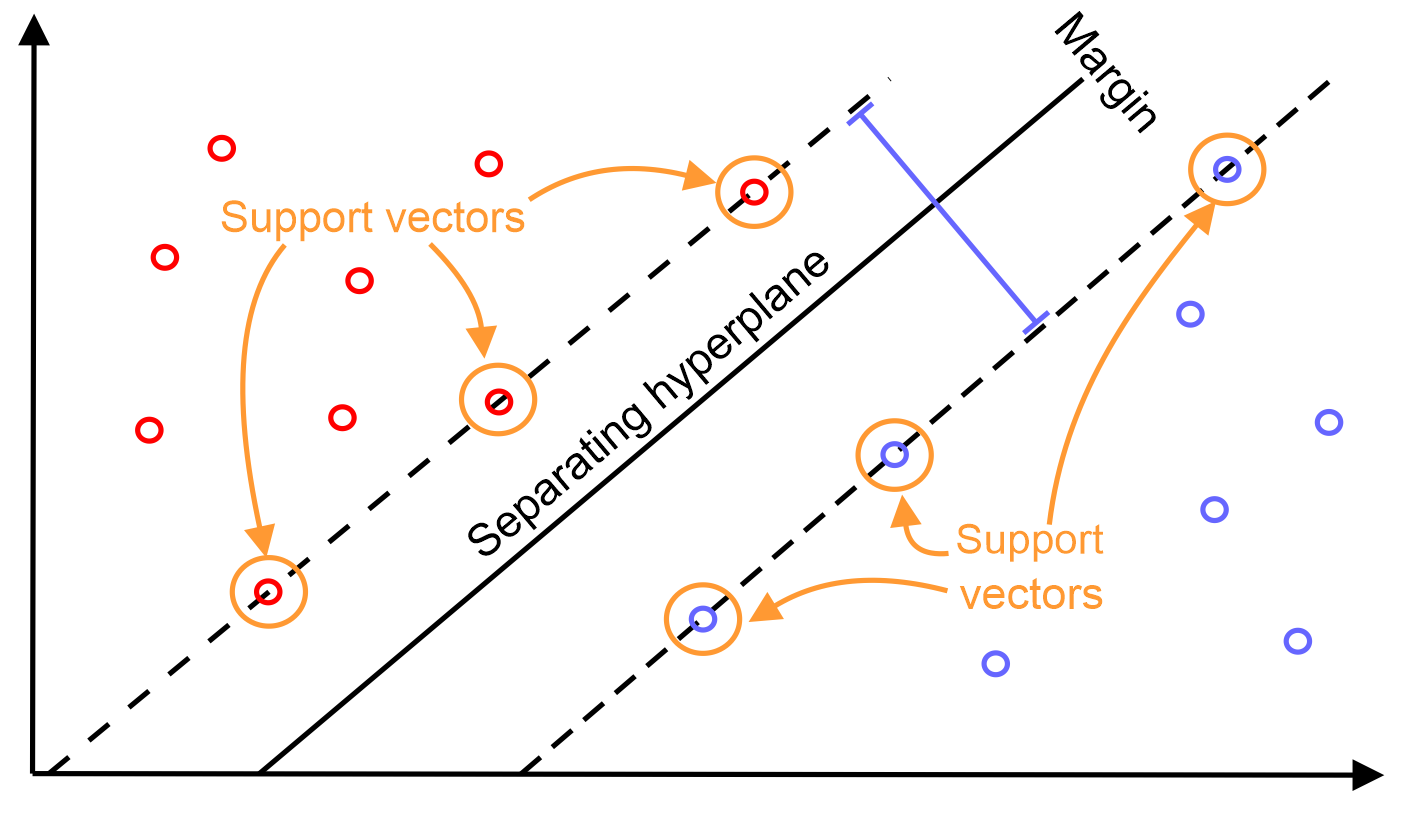
\includegraphics[width=1\linewidth]{images/recognition/howItWorks_svm}
		\captionof{figure}[Graphical representation of SVM.]{The overall mechanics of SVM. The red and blue classes are divided by the hyperplane that maximizes the margin length, defined as the shortest distance from the closest point on both sides.}
		\label{fig:howItWorks_svm}
	\end{minipage}
	\begin{minipage}{.39\textwidth}
		\centering
		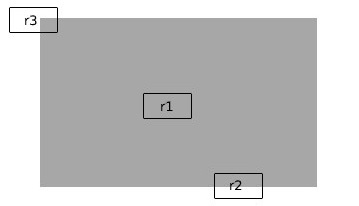
\includegraphics[width=1\linewidth]{images/recognition/kpMatch_regions}
		\captionsetup{margin=0.5cm}
		\captionof{figure}[Three possible regions for key points: flat area, edge or corner.]{Three possible regions that can be used as keypoints. R1 cover a complete flat region. R2 is located on an edge. R3 is placed on a corner, this is the location that can be better recognised.}
		\label{fig:kpMatch_regions}
	\end{minipage}
\end{figure}

\subsection{Key points matching}
The key points, or \textbf{feature points}, matching is a technique that compares two images and tries to recognise which are the common elements of the two. It is widely used to find small patterns in complex images, understand the variation of orientation, stitching panorama view and judge if the subject of two pictures could be the same.\\
This technique is based on key points. These elements are position in the image that can be easily located and identified as unique. In~\Cref{fig:kpMatch_regions} are shown three regions, a flat area, an edge and a corner. The most recognizable point is the one placed at the corner. If an object appears in two images a key point should be recognised in both the appearances.

\subsubsection*{Technique definition and known algorithms}
This technique is divided into two modules:
\begin{itemize}
	\item \textbf{Feature localization}: This module working on a single image at a time, is internally divided into:
	\begin{itemize}
		\item \textbf{Feature detection}: Given the raw image the goal is to identify all the corners that can be easily re-identified in another image.
		\item \textbf{Feature description}: A small area containing few pixels cannot be easily matched. So, the descriptor needs to take each identified key point and normalize them in order to be independent respect to the image conditions like illumination and orientation. This key point enriched with additional information is the feature point.
	\end{itemize}
	A visualization of the feature localization is shown in~\Cref{fig:kpMatch_tesla}.\\
	To solve this task exist several methods were used\footnote{Note that since the mechanics of the methods are similar and this technique has not actually been implemented in the thesis the algorithms reported here are not explained.}:
	\begin{itemize}
		\item \underline{SIFT (Scale-Invariant Feature Transform)}\cite{sift} is able to manage both rotations and scale variation of the feature points.
		\item \underline{SURF (Speeded-Up Robust Features)}\cite{surf} is the advanced version of SIFT with all its pro but, in addition, has a lower processing time and produce an extremely high number of feature points.
		\item \underline{ORB (Oriented FAST and Rotated BRIEF)}\cite{orb} is the only algorithm of the three that is not patented. It is a combination of two sub methods:
		\begin{itemize}[\ding{228}] %method to insert custom symbol in itemize (\ding(228) = the full >)
			\item \underline{FAST (Features from Accelerated Segment Test)}:\cite{fast} method completely focused on pure speed.
			\item \underline{BRIEF (Binary Robust Independent Elementary Features)}\cite{brief} algorithm extremely sensitive to noise, use Gaussian kernels to remove it and work precisely.
		\end{itemize}
	\end{itemize}

	\item \textbf{Feature matching}: The third module of this technique works on two images after that the feature points were computed. The goal is to match the features of the two images together. A match can only be one by one. A feature point should have exactly one corresponding point in the other image and vice versa, to be a correct and reliable connection. If a point is linked to more than one on the other image, this means that the connection works with multiple inaccurate key points hardly recognisable.\\
	In~\Cref{fig:kpMatch_notreDame} is presented an example working on two similar images. All the correct matches, draw as green lines, can be used to both assigns a probability that represents, how likely the subjects are the same "object". But also to understand which type of 3D transformation can be applied to an image to convert it into the other one.\\
	\\
	The existing algorithms for the matching are:
	\begin{itemize}
		\item \underline{BFM (Brute Force Matcher)} This is the naive solution. All the possible combinations of points of the two different images are tried. Obviously is a precise method because it does not work under assumption but if the number of key points is high this method is at all infeasible.
		\item \underline{FLANN (Fast Library for Approximate Nearest Neighbors) matcher}\cite{flann} Differently from BFM, this method is optimized to work even with a large number of features. The optimization is based on the local search of K-Nearest Neighbors.
	\end{itemize}
\end{itemize}
\begin{figure}[!h]
	\centering
	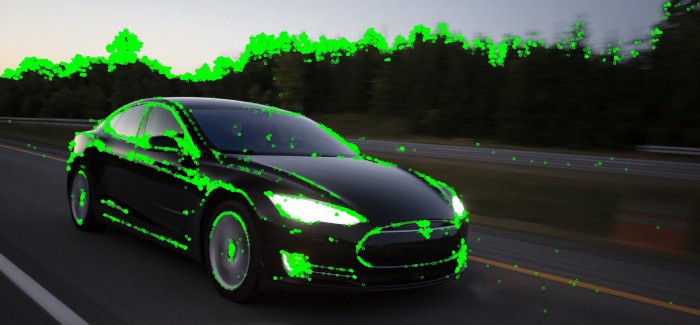
\includegraphics[width=0.7\linewidth]{images/recognition/kpMatch_tesla}
	\captionsetup{margin=0.5cm}
	\caption[Key points localization on a Tesla.]{The feature localization module applied to a Tesla. The key points are spread along the edges of the car and the background. Instead, the road has not, because the patter is often repeated, hence it is not reliable.}
	\label{fig:kpMatch_tesla}
\end{figure}
\begin{figure}[!h]
	\centering
	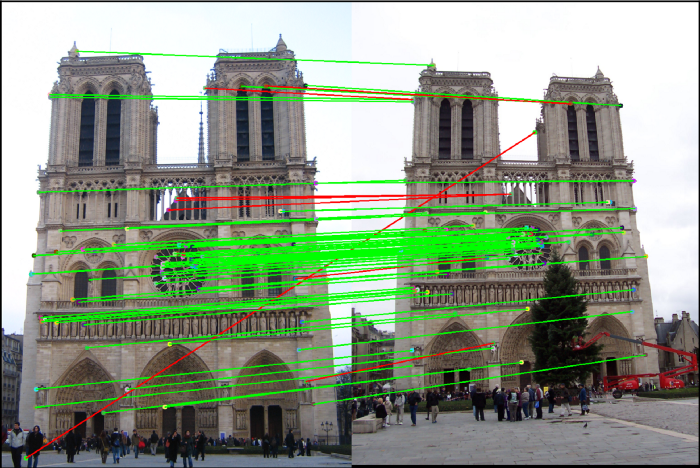
\includegraphics[width=0.7\linewidth]{images/recognition/kpMatch_notreDame}
	\captionsetup{margin=0.5cm}
	\caption[Key points matching with Notre Dame comparison.]{Two images of Notre Dame de Paris are aligned with the feature matcher. Since the image is very clear a lot of points are paired correctly (green lines), while a few of them are not (red lines).}
	\label{fig:kpMatch_notreDame}
\end{figure}

\subsubsection*{Key points matching applied to people}
The initial idea was to apply the key point matching to people. The test were done on the \textbf{PRID450 (Person Re-IDentification)}\cite{prid450} dataset that contains thousands of images of cropped people walking outdoors. The dataset is constructed with multiple shots of the same person on different moment and prospectives.\\
The idea has two big problems:
\begin{itemize}
	\item The images cropped around the people has a very low resolution. The result is that the details that could distinguish a person from another one cannot be visible, or better cannot be recognised.
	\item Humans present a high deformable-body, with a surface (clothes) that continuously change aspect. Instead, the key point matching is designed for a pattern that is repeated often and clearly. The consequence of this is a matching that works as if it were random.
\end{itemize}
In~\Cref{fig:kpMatch_samples} are shown some examples that visually demonstrate the unreliability of this technique applied to humans.

\begin{figure}[!h]
	\centering
	\begin{subfigure}[!h]{0.24\textwidth}
		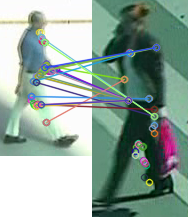
\includegraphics[width=\linewidth]{images/recognition/kpSample_aLotofMatches2}
	\end{subfigure}
	\begin{subfigure}[!h]{0.24\textwidth}
		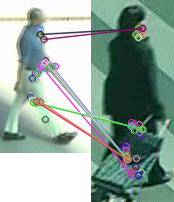
\includegraphics[width=\linewidth]{images/recognition/kpSample_object2}
	\end{subfigure}
	\begin{subfigure}[!h]{0.24\textwidth}
		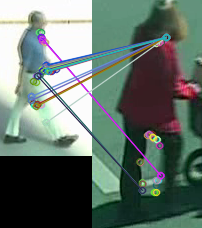
\includegraphics[width=\linewidth]{images/recognition/kpSample_falsePositive}
	\end{subfigure}
	\begin{subfigure}[!h]{0.24\textwidth}
		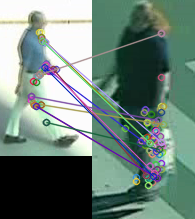
\includegraphics[width=\linewidth]{images/recognition/kpSample_object}
	\end{subfigure}
	%
	\begin{subfigure}[!h]{0.24\textwidth}
		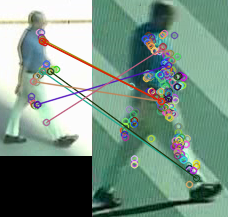
\includegraphics[width=\linewidth]{images/recognition/kpSample_samePerson}
	\end{subfigure}
	\begin{subfigure}[!h]{0.24\textwidth}
		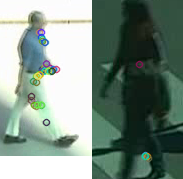
\includegraphics[width=\linewidth]{images/recognition/kpSample_noMatch}
	\end{subfigure}
	\begin{subfigure}[!h]{0.24\textwidth}
		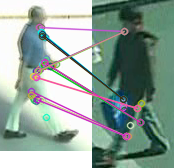
\includegraphics[width=\linewidth]{images/recognition/kpSample_aLotofMatches}
	\end{subfigure}
	\begin{subfigure}[!h]{0.24\textwidth}
		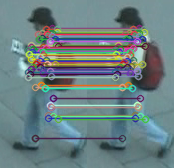
\includegraphics[width=\linewidth]{images/recognition/kpSample_self}
	\end{subfigure}
	\captionsetup{margin=0.5cm}
	\caption[Key points matching samples of people comparison.]{Some matching samples show that key point matching easily fails under these conditions. There are multiple wrong aspects: people that present no key points, objects such as bags that have plenty of features, matching that connects completely different parts of the body like shoulders with legs. Even with the same subject with almost the same position (bottom-left images), the algorithm fails with most of the points. The exception is the bottom-right image that has a perfect matching, but the two pictures are exactly the same one. So it is not a reliable test.}
	\label{fig:kpMatch_samples}
\end{figure}


\section{KNN (K-Nearest Neighbors) with images into N-dimensional space}\label{sec:knn}
Since that offline algorithms cannot be used, the official solution is based on online algorithms. The chosen method is KNN (K-Nearest Neighbors) classifier is a widely used method that is based on the proximity of points into space, where each point has a class. When a new point should be judged, the K nearest known points are found, and the class for the new incoming is chosen according to the majority of classes of the K selected points (an example is shown in~\Cref{fig:howItWorks_knn}).\\
About this algorithm, some aspect should be considered:

\begin{itemize}
	\item KNN is a native online method. The difference between online and offline is about computing the training in advance or not, but KNN has no training phase. The training only requires to store the known points with the associated labels, and this is done at almost no cost.
	\item The elaboration works with points and not images, this remarkably reduces the computational classification cost.\\
	On the other hand, an image should be collapsed to a point, meaning that a good representation should be used to do not lose important information.
	\item The classification steps should compare the new cropped frame, transformed into a point, with all the other known points. So, a very high number of stored points will slow down the execution. But in our real-time scenario, this will occur only if the tracking will last for an extremely long period, and this will not happen.
\end{itemize}
To apply KNN, the challenging task of converting images into representative points should be solved.
\begin{figure}
	\centering
	\begin{minipage}{.44\textwidth}
		\centering
		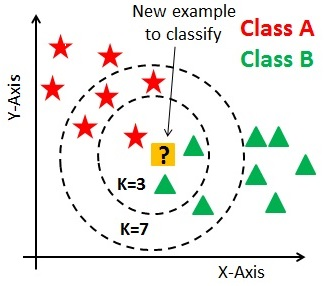
\includegraphics[width=1\linewidth]{images/recognition/howItWorks_knn}
		\captionsetup{margin=0.5cm}
		\captionof{figure}[Example of application of the KNN classifier.]{Example of the mechanics of KNN. The new point (question mark) will be classified as class $B$ if the 3 nearest neighbours are considered. It will be classified as class $A$ if K=7 is used.}
		\label{fig:howItWorks_knn}
	\end{minipage}
	\begin{minipage}{.54\textwidth}
		\centering
		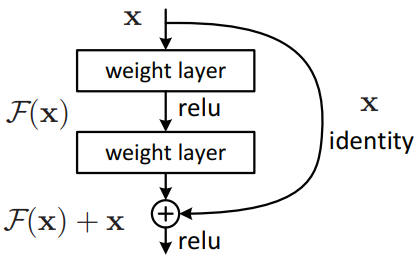
\includegraphics[width=1\linewidth]{images/recognition/howItWorks_resNet}
		\captionsetup{margin=0.5cm}
		\captionof{figure}[The residual block of ResNet.]{The residual block of ResNet. The identity connection allow to the output of the precedent level, to skip two convolution layers. The result $f(x)+x$ is the combination of the convolutions $f(x)$ combined with the identity $x$.}
		\label{fig:howItWorks_resNet}
	\end{minipage}
\end{figure}


\subsection{Image classifiers for representative points from images} \label{sec:classifiers}
We have chosen to use CNN to create the representative points that should describe an entire image. Unlikely, it does not exist an explicit field of study that aims to create this kind of points. The solution relies into the adaptation of a widely explored machine learning challenge called \textbf{image classification} (\Cref{fig:imgAnalysisType}). The goal is to predict which kind of elements exist inside the picture.\\
The image classifiers based on CNN work as follows:
\begin{enumerate}
	\item The input picture is resized to standard dimensions. In addition, colours and lights are normalized.
	\item The image is elaborated with multiple blocks of convolution's layers.
	\item All the features extracted with the convolutions are collapsed, with a "\textit{flatten operation}", into an array of thousands of elements.
	\item In the end, this vector is eventually reduced and the final predictions, one for each output class, are generated.
\end{enumerate}
The goal is to generate a point from the input image of CNN. The fourth part collapses all the elaborated information into predictions that vary according to the context of the application. Instead, the third level produces an array: a list of N numbers that can be seen as coordinates of a point into an \textbf{N-dimensional space}. KNN works independently from the space dimensionality, so, it does not matter how many features are produced the CNN based algorithms.\\
\\
The classifier chosen are the DNNs (Deep Neural Networks) \textbf{GoogLeNet} and \textbf{ResNet}\cite{resNet_model}. A DNN has the capability to produce better results than a NN. On the other hand, the huge number of parameters used should be tuned during the training phase. This calibration of the values is extremely hard on small datasets due to the \textbf{vanishing gradient problem}. Therefore, both classifiers introduce a novelty aiming to solve the problem connected to the depth of the network.

\subsubsection*{ResNet (Residual Network)}
ResNet\cite{resNet_paper} is build on top of the idea of "skip blocks of layers". The residual block is shown in~\Cref{fig:howItWorks_resNet}.\\
A "\textit{plain CNN}" has convolutions stacked one after the other, in this case, there is an additional element: the \textbf{identity connection}. It means that no filters are applied, the input is shifted two layers down. This connection is used to propagate the information deep into the CNN without modifying them. The advantage is that the input image is preserved through the network and it is not affected by an elaboration that lasts for several layers (more than 100). This novelty is very important for small training sets that are not able to fine-tune all millions of parameters of the DNN.\\
The original paper comes out with multiple models characterized by different depths, for this thesis we have chosen ResNet50\cite{resNet_model}. This model produces a representation point in 2048 dimensions.

\subsubsection*{GoogLeNet (Google Le-Network)}
GoogLeNet\cite{googLeNet_paper} is based on a new convolution scheme called \textbf{Inception module}. The name and the goal of module comes from the quote “\textit{We need to go deeper}”\footnote{Quote of the film Inception (\href{https://i.kym-cdn.com/photos/images/newsfeed/000/531/557/a88.jpg}{meme})}.\\
The naive version of the inception module parallelizes three different convolution filters (1x1, 3x3, 5x5) and a \textit{max-pooling filter}. This special elaboration reduces the depth of the CNN while preserving its potentiality. On the other hand, the number of parameters is still huge. The official version of the inception module (\Cref{fig:howItWorks_inceptionModule}) stacks each filter (3x3, 5x5 and max-pooling) with a 1x1 convolution to reduce, by a factor of 10, the overall number of parameters.\\
We have used the model\cite{googleNet_model} proposed together with the paper. This GoogLeNet implementation produce a representation point in 1024 dimensions (half of ResNet50).
\begin{figure}[!h]
	\centering
	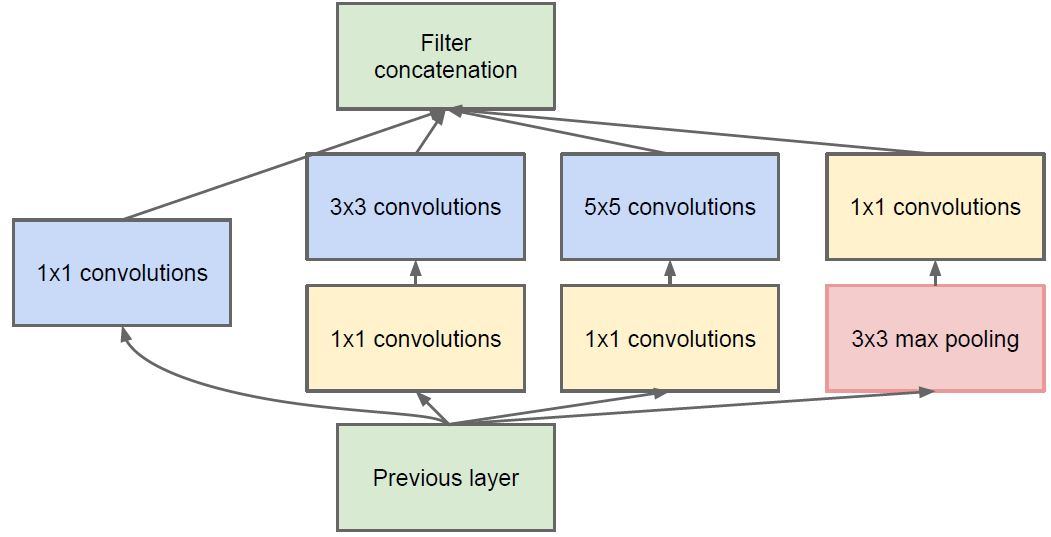
\includegraphics[width=0.8\linewidth]{images/recognition/howItWorks_inceptionModule}
	\captionsetup{margin=0.5cm}
	\caption{The inception module presented with the GoogLeNet model.}
	\label{fig:howItWorks_inceptionModule}
\end{figure}

\subsubsection*{SSP-ReID (Saliency-Semantic Parsing Re-IDentification)}
SSP-ReID\cite{ssp_reID} is a useful technique specifically designed for improving the potentialities of the image classifiers when are applied to bounding boxes of people. This method is ideated to create a representative array of features.\\
The model is based on a "\textit{CNN backbone}" that can be selected from a wide set of pre-existing CNNs such as ResNet or GoogLeNet. The improvement comes from additional pieces of information that are processed together with the backbone.\\
The extra information generated (shown in~\Cref{fig:howItWorks_sspReID}) are:
\begin{itemize}
	\item \textbf{Saliency} (\Cref{fig:sub_saliency}): this technology aims at isolating all the pixels that appear at "first glance" to the human eyes. The set of these pixels are the one that may highlight some key aspects of a person such as a bag, the clothes or other.
	\item \textbf{Semantic Parsing} (\Cref{fig:sub_semanticParsing}): the body of the person is divided into 5 sections and these are elaborated separately. Each body part can have its own characteristics.\\
	The 5 sections are: head, upper body, lower body, shoes and complete body.
\end{itemize}
This method is not integrated into the thesis project at the moment but it can be a great choice for future improvements.

\begin{figure}[!h]
	\centering
	\begin{subfigure}{0.33\textwidth}
		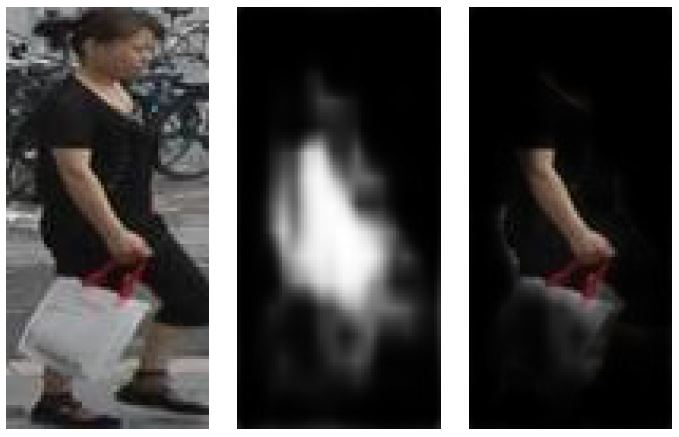
\includegraphics[width=\linewidth]{images/recognition/ssp_saliency}
		\caption{The saliency elaboration, applied to the woman, highlight the presence of a bag.}
		\label{fig:sub_saliency}
	\end{subfigure}
	\begin{subfigure}{0.66\textwidth}
		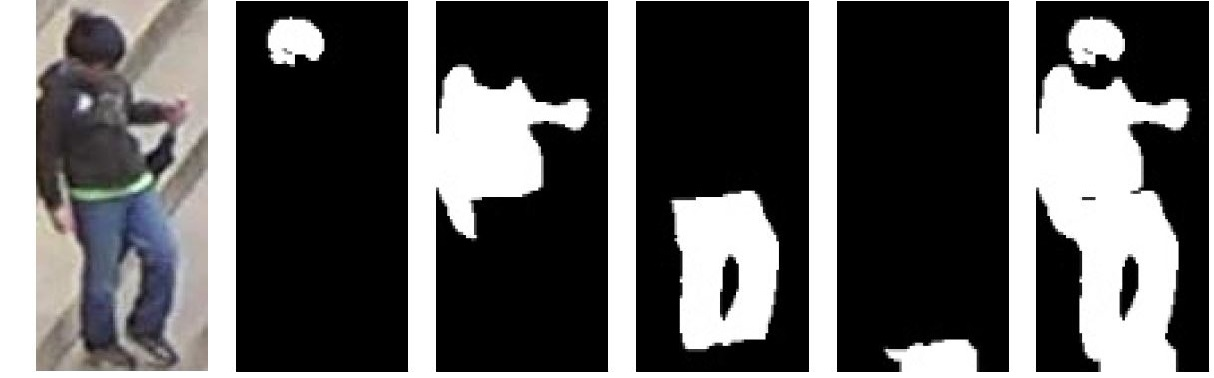
\includegraphics[width=\linewidth]{images/recognition/ssp_semanticParsing}
		\captionsetup{margin=0.5cm}
		\caption{The semantic parsing elaboration divides the body of the child in the 5 sections: head, upper body, lower body, shoes and complete body.}
		\label{fig:sub_semanticParsing}
	\end{subfigure}
	\captionsetup{margin=0.5cm}
	\caption{Examples of saliency and semantic parsing elaborations.}
	\label{fig:howItWorks_sspReID}
\end{figure}

\subsection{Examples of KNN applied to people recognition}
The intuition of using KNN has been tested on the \textbf{Market1501}\cite{market1501} dataset. Similarly to the PRID450 dataset, also this dataset contains sets of images captured from different prospectives and in different moments of hundred of people. Each real person has is own ID so different images of the same subject are associated to the same ID.\\
A couple of the results of the experiments are shown in~\Cref{fig:knn_reID_examples}. This elaboration is done by selecting small datasets of $18$ and $99$ images, of $2$ and $11$ people respectively each one with $9$ pictures per person. KNN was "trained"\footnote{The training of KNN consists of storing data and nothing more.} with the representative points extracted from the images of the datasets. Then, the queries (images of people) were used to retrieve the most similar people. This was done by generating the representative points of the queries and for each one, the K closest points are retrieved together with the associated images.\\
\\
It is important to focus on the ratio between correct and wrong responses, green and red respectively. In the test elaborated with ResNet50 (\Cref{fig:knn_resNet_s9n99}) there are almost 50\% and 50\% of wrong and correct responses, while in the test elaborated with GoogLeNet (\Cref{fig:knn_googleNet_s9n18}) there is only one false prediction over $14$. Despite the different algorithms used the results is independent of them.\\
In fact, the key difference is that in~\Cref{fig:knn_resNet_s9n99} there are 11 classes, so $9*1=9$ samples of the correct person and $9*10=90$ of the wrong one. While in~\Cref{fig:knn_googleNet_s9n18} there are only 2 classes so $9$ samples against $9$. This different ratio between positive and negative training examples affect the result of the predictions.\\
In this thesis, we are dealing only with $2$ classes: the Leader and the other people. Hence, we are interested in the scenario with $18$ images that works extremely well.\\
\\
Lastly, for the integration of person recognition, with the tracking and detection modules, we only need to know if the query belongs to a class or to another one. This choice is based on the most likely class on the first K\footnote{In case of 2 classes K is often chosen odd.}  nearest neighbours of the query, so if the majority is green or red.

\begin{figure}[!h]
	\centering
	\begin{subfigure}{1\textwidth}
		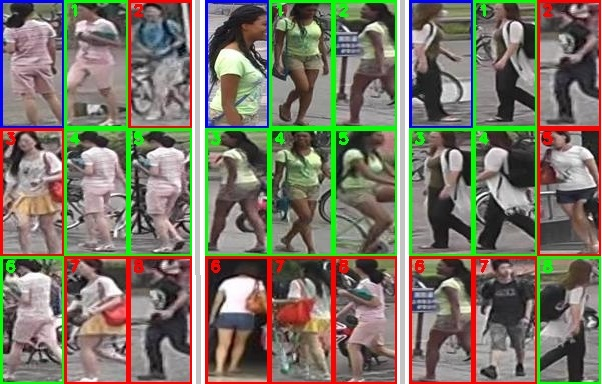
\includegraphics[width=\linewidth]{images/recognition/knn_resNet_s9n99}
		\captionsetup{margin=0.5cm}
		\caption{KNN applied on images elaborated with ResNet50. The training was done with 11 real people and 9 images of each one, for a total of 99 pictures. Here are shown 3 queries with the 8 most similar people.}
		\label{fig:knn_resNet_s9n99}
	\end{subfigure}
	\par\bigskip %vertical spacing
	\begin{subfigure}{1\textwidth}
		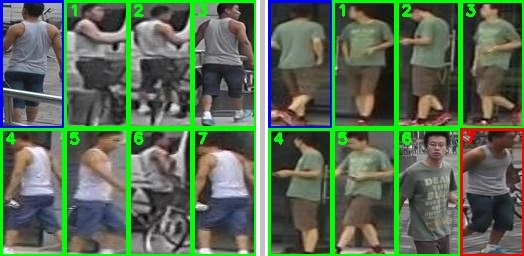
\includegraphics[width=\linewidth]{images/recognition/knn_googleNet_s9n18}
		\captionsetup{margin=0.5cm}
		\caption{KNN applied on images elaborated with GoogLeNet. The training was done with 2 real people and 9 images of each one, for a total of 18 pictures. Here are shown 2 queries with the 7 most similar people.}
		\label{fig:knn_googleNet_s9n18}
	\end{subfigure}
	\captionsetup{margin=0.5cm}
	\caption[KNN applied with image classifier to solve the person re-identification task.]{In this picture are shown queries computed on the KNN classifier that has pre-processed small datasets of images of people. The query (top-left bounding box with blue contour) is used to extract from the database the most similar 7/8 pre-analysed people. The green contour means that the extracted person is correct, while if it is wrong the red is used.}
	\label{fig:knn_reID_examples}
\end{figure}